
\documentclass[a4paper]{article}
\usepackage{pslatex}
\usepackage[T1]{fontenc}
\usepackage[utf8x]{inputenc}
\setlength\parskip{\medskipamount}
\setlength\parindent{0pt}
\usepackage{graphicx}
\usepackage{amssymb}
%\usepackage{hyperref}

\usepackage{multicol}

\makeatletter

\providecommand{\boldsymbol}[1]{\mbox{\boldmath $#1$}}
\newcommand{\ASL}			{ASL}
\newcommand{\OSC}[1]		{\texttt{#1}}
\newcommand{\lra}			{$\leftrightarrow$}
\newcommand{\seg}[1]		{Seg(#1)}

\setlength{\parskip}{1mm}

\makeatother

\begin{document}

\title{FaustLive - Specification \\ v.1.2}

\author{Grame, Centre National de Création Musicale\\
{\small <research@grame.fr>} \\
\vspace{2mm}
[ANR-12-CORD- 0009] and [ANR-13-BS02-0008]
}

\maketitle

\topskip0pt

\vspace{\fill}

%==================================================================================================
FaustLive is an advanced self-contained prototyping environment for the Faust programming language with an ultra-short edit-compile-run cycle. Thanks to its fully embedded compilation chain, FaustLive is simple to install and doesn't require any external compiler, development toolchain or SDK to run. FaustLive is the ideal tool for fast prototyping. Faust programs can be compiled and run on the fly by simple drag and drop. They can even be edited and recompiled while running without sound interruption or Jack disconnection. \\
\\
FaustLive is based on QT. Most classes are a reimplementation of QObjects. 
To know more about these base-objects, see QT documentation : http://qt-project.org/doc/qt-5/classes.html
\vspace{\fill}

\newpage
\tableofcontents

\newpage
\section{General Considerations}

The structure of FaustLive is based on three main classes : FLApp, FLWindow and FLSessionManager.

\begin{itemize}
\item FLApp is a reimplementation of QApplication. Its role is to be a communication center between the menus, dialogs, windows, etc. 

\item FLWindow reimplements QMainWindow. Its role is to contain the DSP, its interface(s) and react to the window's menus/actions/...

\item FLSessionManager is a simple QObject. Its role is to be the compilation center and maintain the hierarchy of the current session. 

\end{itemize}

Many of the dialogs and internal structure classes are singletons to share their information with one shared access point. 

%%%%%%%%%%%%%%%%%FAUSTLIVE APP%%%%%%%%%%%%%%%%%%%
\section{FLApp}
 
FLApp reimplements QApplication. For that matter, it contains the main event loop, where all events from the window system and other sources are processed and dispatched. It also handles the application's initialization (some singletons have to be initialized by FLApp) and finalization.

\subsection{Menus}

The menus are handled differently, depending on the platform. \\
On OSX, the menu of the application appears in the system external menu-bar. Depending on the front window, the specific menus will show. \\
On Windows and Linux, each window of the application has its own menu-bar. There is no general menu-bar. That is why, when the last window is closed, the application quits : no more actions are available. \\

While some actions are specific to the windows (edit, export, ...), others  are to be treated by the application (new, open, ...). The application-related menus and actions have to be created by the application to be connected to its SLOT. When a window is created, it receives its menus created by the application. 

So, FLApp contains the following functions :
\begin{itemize}
\item create\_FileMenu() : QMenu* 
\item create\_ExampleMenu() : QMenu*
\item create\_RecentFileMenu() : QMenu*
\item create\_NavigateMenu() : QMenu*
\item create\_HelpMenu() : QMenu*
\end{itemize}

\subsection{Create FLWindow}

To create a new FLWindow, the application has to choose two things
- The index of the window (the smallest not currently used)
- The position (depending on the index)

\subsection{Menus and Dialogs}

Help Dialog


\subsubsection{}
%%%%%%%%%%%%%%%%%WINDOW%%%%%%%%%%%%%%%%%
\section{FLWindow}

%%%%%%%%%%%%%%%%%SESSION MANAGER%%%%%%%%%%%%%%%%%
\section{FLSessionManager}

FLSessionManager is a singleton.\\

The role of FLSessionManager is to be the link with libfaust and libfaustremote, to compile the DSPs. Moreover, it has the function to maintain the hierarchy of the current session and be able to save/recall sessions and snapshots. 

\subsection{Current Session Hierarchy}

The current session is composed of : 
\begin{itemize}
\item Settings.ini : file containing the saved settings as described in FLSettings
\item Examples : folder containing a copy of the example files of the faust distribution
\item Libs : folder containing a copy of the libraries of the faust distribution
\item Windows : folder containing the window-specific folders FLW-i, containing :
	\begin{itemize}
		\item Settings.ini : the window specific settings as described in FLWinSettings
		\item Graphics.rc : file saving the graphical parameters of the last DSP contained in the window
		\item Connections.jc : file saving the last known Jack connections of the window
		\item SHAKey.dsp : copy of the faust code of the last DSP contained in the window (in case the original file is deleted or modified outside of FaustLive execution)
	\end{itemize}
\item SHAFolder : folder containing the DSP-specific folders, containing : 
	\begin{itemize}
		\item SHAKey : LLVM intermediate representation of the DSP, to accelerate compilation when the same DSP is reused.
		\item SHAKey.dsp : copy of the Faust code corresponding to this SHAKey
		\item SHAKey-svg : folder containing the svg diagram resources
	\end{itemize}
\end{itemize}


\subsection{DSP compilation}

To compile a DSP, there are two steps :
\begin{itemize}
\item create a factory (builds the protoype of a the DSP class)
\item create an instance of the factory (equivalent of a 'new class" in C++)
\end{itemize}

Because FaustLive enables remote processing, the factories and instances it creates can whether be local (llvm\_dsp\_factory / llvm-dsp ) through libfaust or remote (remote\_dsp\_factory / remote-dsp) through libfaustremote. \\

The goal of FLSession Manager is to be the only class that deals with remote\_dsp\_factory, llvm\_dsp\_factory, remote-dsp, llvm-dsp, ...

The classes that will need compilation will only receive a pointer to a dsp, without knowing its type. \\

Still, the two steps cannot be united in the same function, because some audio initialization is needed between the two steps (for the remote case where the sample rate and buffer size are needed to create the instance and only available once the factory is created...).

In conclusion, to create a dsp, you have to call :
\begin{itemize}
\item createFactory(const QString\& source, QString\& errorMsg, FLWinSettings* settings = NULL) : returns QPair<QString, void*> ;
\item createDSP(QPair<QString, void*> factorySetts, const QString\& source, QString\& errorMsg, FLWinSettings* settings = NULL, RemoteDSPErrorCallback error\_callback = NULL, void* error\_callback\_arg = NULL) : returns dsp*;
\end{itemize}

\subsubsection{create Factory}

Depending on the machine name, 

\subsubsection{create Instance}

\subsection{Session/Snapshot restoration}

%%%%%%%%%%%%%%%%%SETTING STRUCTURE%%%%%%%%%%%%%%%%
\section{Setting Management}

%%%%%%%%%%%%%%%%%GENERAL SETTINGS%%%%%%%%%%%%%%%%%
\subsection{FLSettings}

FLSettings is a singleton. 
To save settings, the class FLSettings reimplements QSettings. A hierarchy, presented {Figure \ref{fig:FLSettings}, allows us to access the settings easily. \\

The setting file is saved at the root of the current session (/Users/you/.FaustLiveCurrentSession-version).

\begin{figure}[!h]
\begin{center}
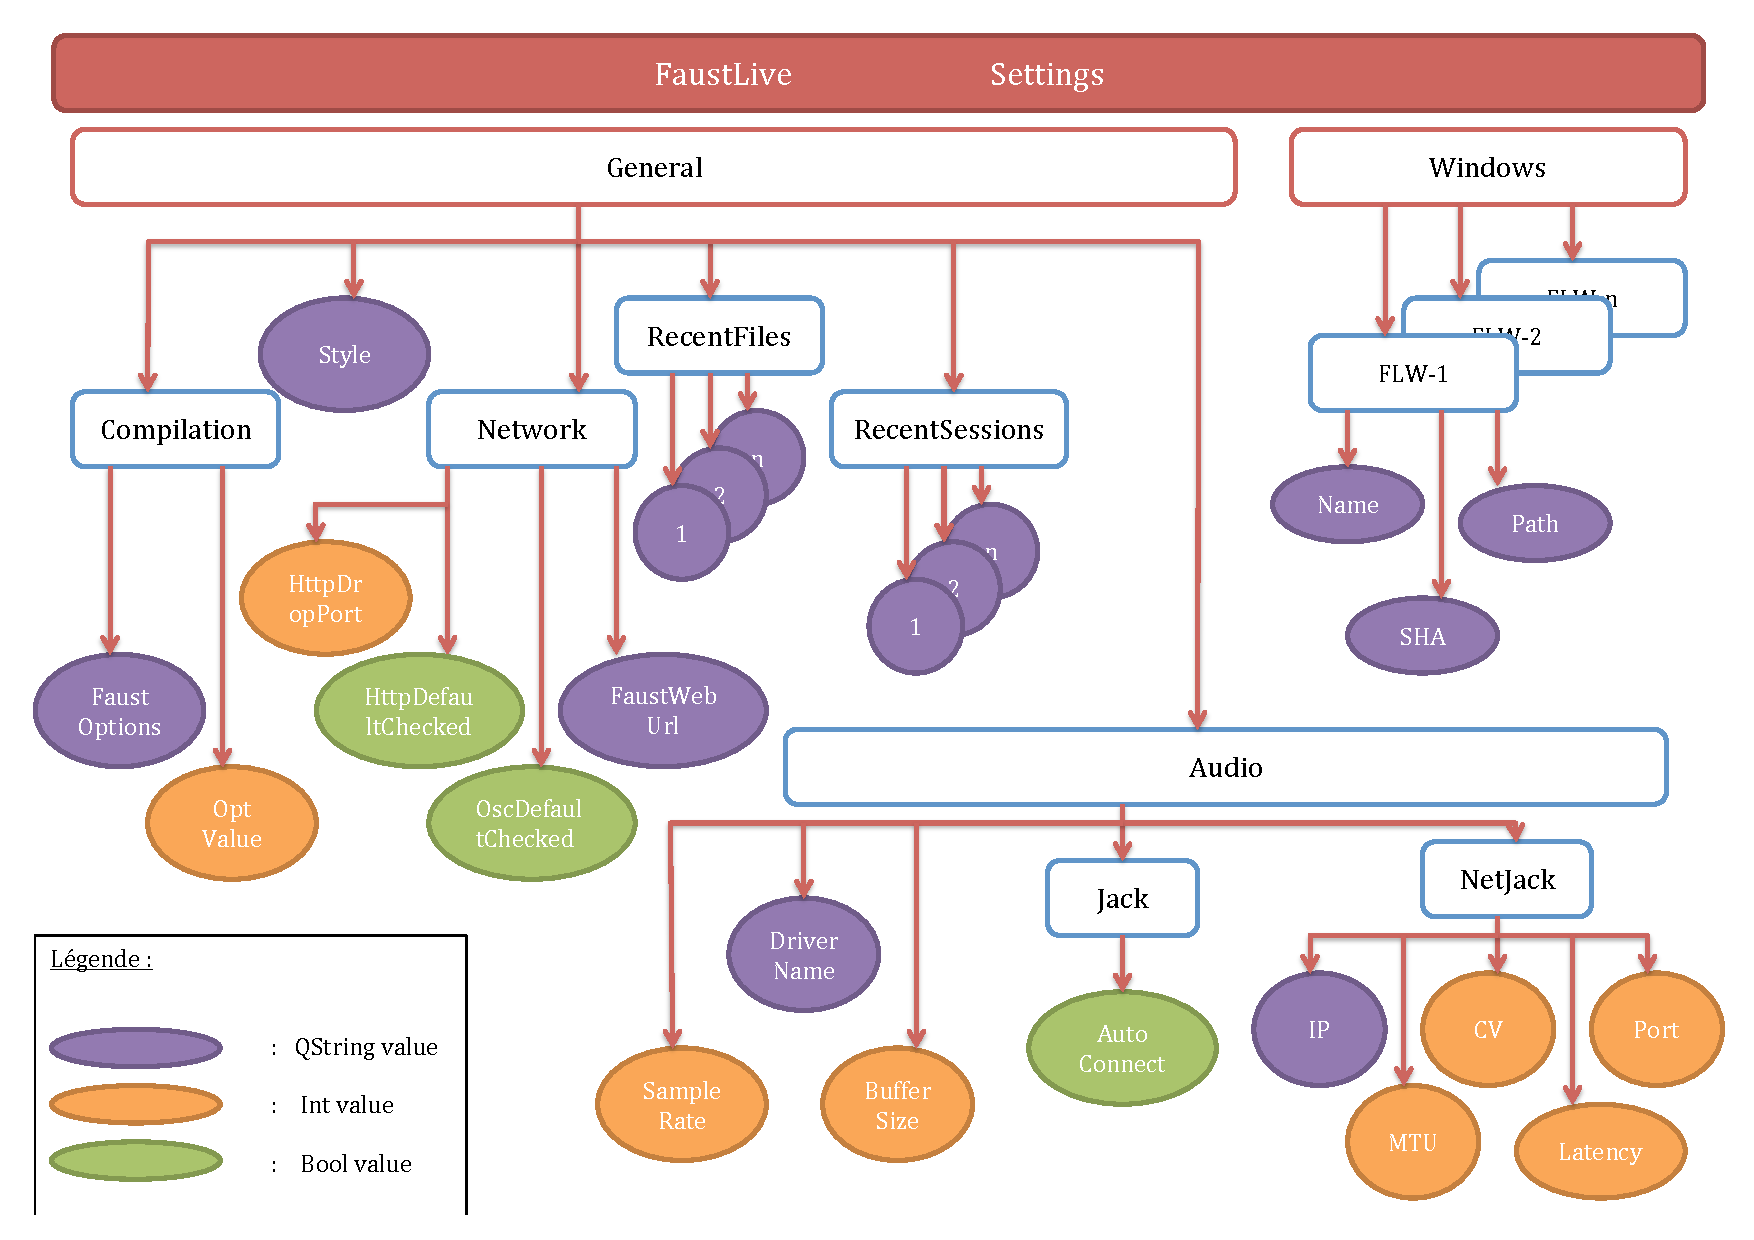
\includegraphics[width=\columnwidth]{images/FLSettings}
\caption{FLSettings structure}
\label{fig:FLSettings}
\end{center}
\end{figure}

\begin{multicols}{2}
\begin{itemize}
\item General
	\begin{itemize}
	\item Compilation
		\begin{itemize}
		\item FaustOptions <QString>
		\item OptValue <Int>
		\end{itemize}
	\item Style <QString>
	\item Network
		\begin{itemize}
		\item FaustWebUrl <QString>
		\item HttpDropPort <Int>
		\item HttpDefaultChecked <Bool>
		\item OscDefaultChecked <Bool>
		\end{itemize}
	\item RecentFiles
		\begin{itemize}
		\item 1/2/.../n <QString>
		\end{itemize}
	\item RecentSession
		\begin{itemize}
		\item 1/2/.../n <QString>
		\end{itemize}
	\item Audio
		\begin{itemize}
		\item DriverName <QString>
		\item SampleRate <Int>
		\item BufferSize <Int>
		\item Jack
			\begin{itemize}
			\item AutoConnect <Bool>
			\end{itemize}
		\item NetJack
			\begin{itemize}
			\item IP <QString>
			\item MTU <Int>
			\item CV <Int>
			\item Latency <Int>
			\item Port <Int>
			\end{itemize}
		\end{itemize}
	\end{itemize}
\item{Windows}
	\begin{itemize}
	\item FLW-i
		\begin{itemize}
		\item Name <QString>
		\item SHA <QString>
		\item Path <QString>
		\end{itemize}
	\end{itemize}
\end{itemize}
\end{multicols}

 
For example, you can access the value like this :\\
\textit{int httpPort = FLSettings::\_Instance()->value("General/Network/HttpDropPort", defaultValue);}

%%%%%%%%%%%%%%%%%WINDOW SETTINGS%%%%%%%%%%%%%%%%%
\subsection{FLWinSettings}

FLWinSettings reimplements QSettings. But, this class is not a singleton, each FLWindow is associated to a FLWinSettings. 

\begin{figure}[!h]
\begin{center}
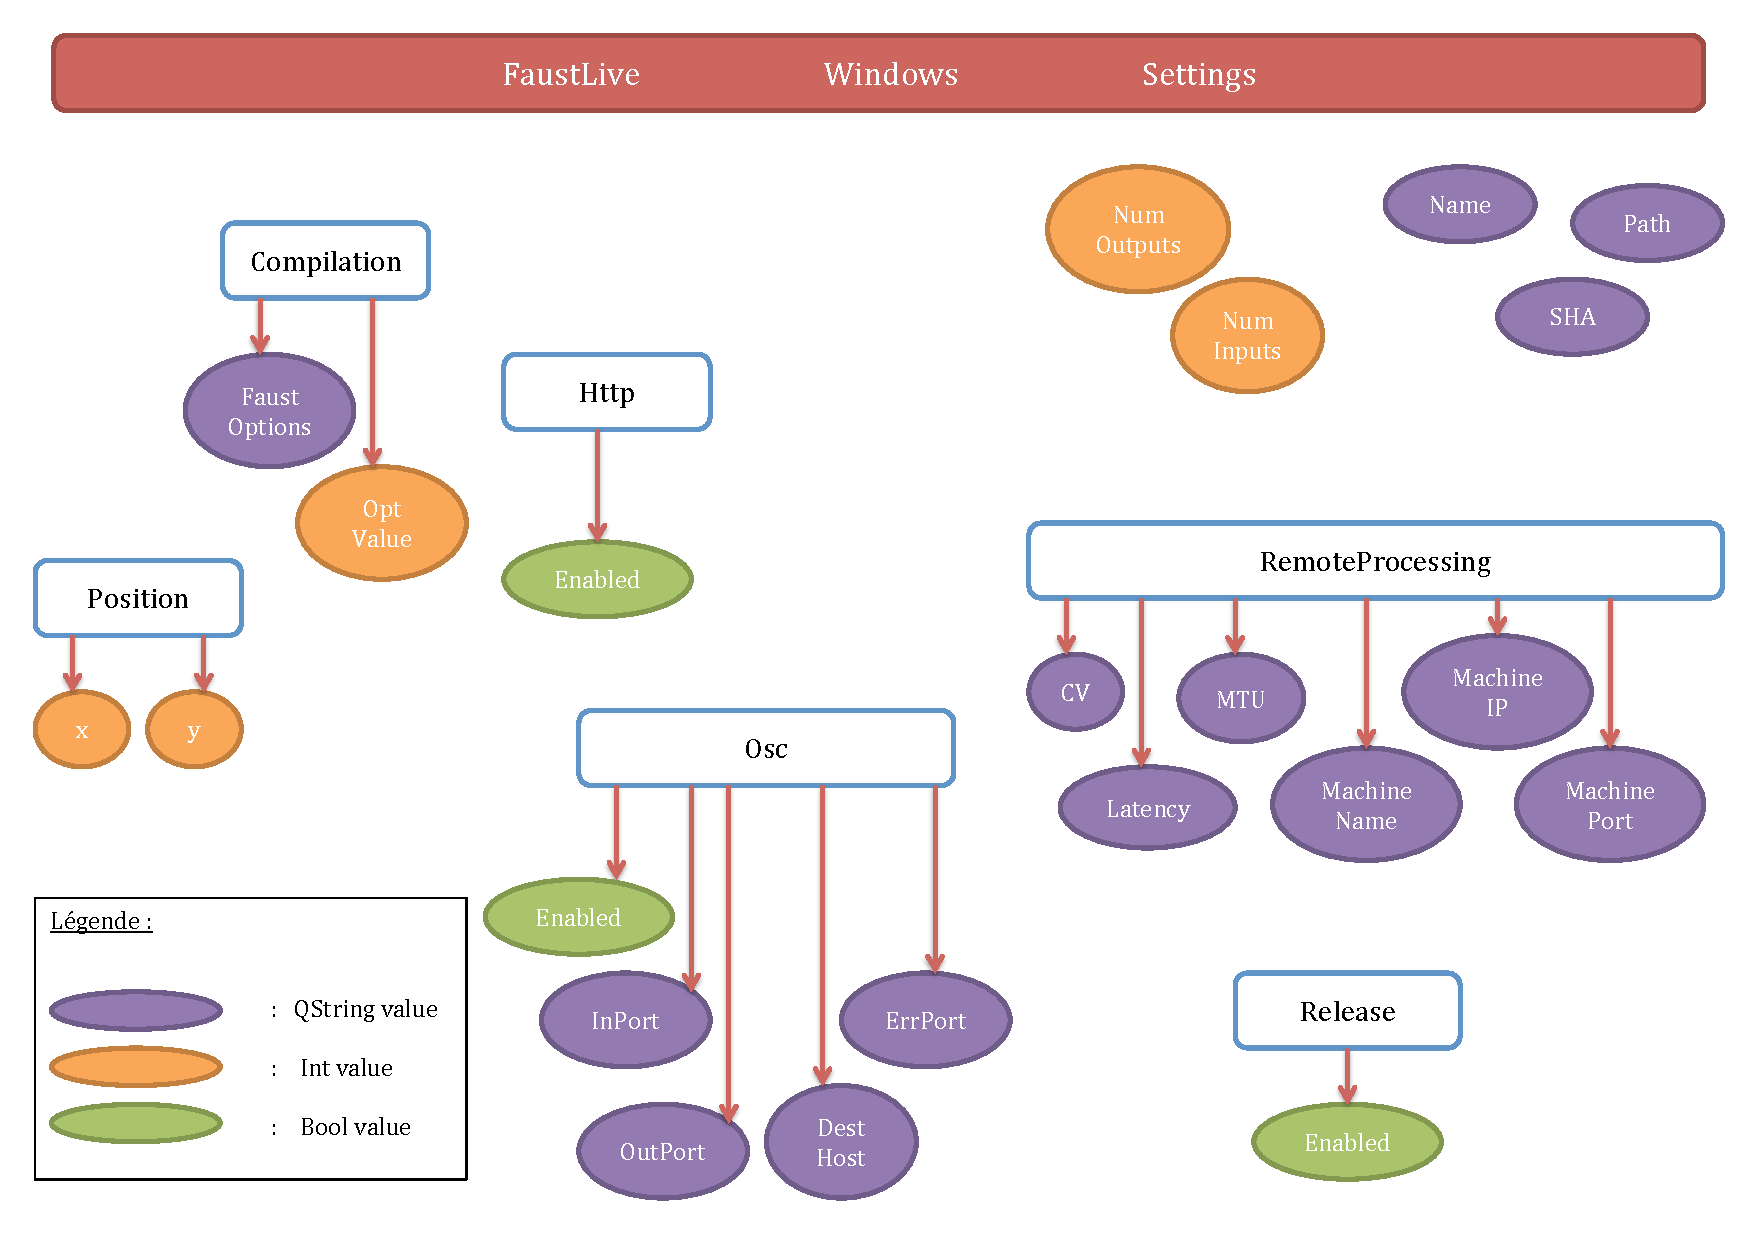
\includegraphics[width=\columnwidth]{images/FLWinSettings}
\caption{FLWinSettings structure}
\label{fig:FLWinSettings}
\end{center}
\end{figure}

\begin{itemize}
\begin{multicols}{2}
\item NumOutputs <Int>
\item NumInputs <Int>
\item Name <QString> ***
\item SHA <QString> ***
\item Path <QString> ***

\item Compilation
	\begin{itemize}
		\item FaustOptions <QString>
		\item OptValue <Int>
	\end{itemize}

\item Http
	\begin{itemize}
		\item Enabled <Bool>
	\end{itemize}
	
\item Position
	\begin{itemize}
		\item x <Int>
		\item y <Int>
	\end{itemize}
	
\item Osc
	\begin{itemize}
		\item Enabled <Bool>
		\item InPort <QString>
		\item OutPort <QString>
		\item ErrPort <QString>
		\item DestHost <QString>
	\end{itemize}
	
\item Release
	\begin{itemize}
		\item Enabled <Bool>
	\end{itemize}
	
\item RemoteProcessing
	\begin{itemize}
		\item CV <QString>
		\item MTU <QString>
		\item Latency <QString>
		\item MachineName <QString>
		\item MachineIP <QString>
		\item MachinePort <QString>
	\end{itemize}
		
\end{multicols}
\end{itemize}

For example, you can access the value like this :\\
\textit{int oscInPort = fSettings->value("Osc/InPort", defaultValue);} \\

 *** The added feature of FLWinSettings, compared to QSettings, is to synchronize three parameters of the window with the general settings. That way, Name, SHA and Path are accessible from the general settings. This feature is really usefull for snaspshot and session restoration, to have a global vision of the existing windows.

%%%%%%%%%%%%%%%%%AUDIO STRUCTURE%%%%%%%%%%%%%%%%%
\section{Audio}

\subsection{Audio drivers used by FaustLive}
 
Depending on the operating system and the compiling options, it is possible to embed different audio architectures to FaustLive.
Default drivers are :
- Coreaudio on OSX
- Jack on Linux
- Portaudio on Windows

Then Jack, NetJack and PortAudio can be added with make options : JACK=1 NETJACK=1 PORTAUDIO=1.

\subsection{Code Organisation}
--> General
--> Crossfade
--> 

\subsection{How to add a new audio architecture}

1) Implement the classes : \\
	- audioFader\\
	- audioFactory\\
	- audioManager\\
	- audioSettings\\

2) Modify AudioCreator to add the architecture in\\
	- enum audioArchitecture\\
	- add item in fAudioArchitecture\\
	- add case in createFactory\\
	- add case in read/write Settings\\

3) Modify FaustLive.pro to add the libraries through conditional Compilation


\section{Distribution Structure}

--> Build Folder with targets
--> 


\subsection{Create a new distribution}

--> 







\end{document}




